\documentclass{article}
\usepackage{amsmath}
\usepackage{amsfonts}
\usepackage{amsthm}
\usepackage{centernot}
\usepackage{tikz}
\usetikzlibrary{automata,positioning,arrows.meta}
\usepackage[utf8]{inputenc}
\usepackage{forest}

\newtheorem{innercustomthm}{Theorem}
\newenvironment{customthm}[1]
  {\renewcommand\theinnercustomthm{#1}\innercustomthm}
  {\endinnercustomthm}

\theoremstyle{definition}
\newtheorem{definition}{Definition}

\author{Mostafa Hassanein}
\title{Theory of Language Translation (MTH683) Finals Questions Bank}
\date{11 Jan 2026}
\begin{document}

\maketitle

\newpage

\section*{3-1}
\textbf{Regular Definitions}

Give a regular definition for non-negative integers without leading zeros. A zero is represented by a single 0.

\begin{center}
  \underline{Solution:}
\end{center}

Let:
\begin{itemize}
    \item[] $P_1 = \langle digit, [0-9]\rangle$
    \item[] $P_2 = \langle nonzero\_digit, [1-9]\rangle$
    \item[] $P_3 = \langle number, 0 \mid nonzero\_digit (digit)^* \rangle$
\end{itemize}

The regular definition is given by the sequence:
\begin{align*}
  \langle P_1, P_2, P_3 \rangle.
\end{align*}


Alternatively:

\begin{itemize}
    \item[] $digit \rightarrow [0-9]$
    \item[] $nonzero\_digit \rightarrow [1-9]$
    \item[] $number \rightarrow 0 \mid nonzero\_digit (digit)^{*}$
\end{itemize}

\newpage
% ---

\section*{3-2}
\textbf{Action-Augmented Regular Definitions}

For the following action-augmented regular definition, give a regular expression describing the language of possible outputs. Assume that all inputs are strings of 0's and 1's only

\begin{align*}
  5 &\rightarrow 0  &\text{printf("c")} \\
  6 &\rightarrow 00 &\text{printf("a")} \\
  7 &\rightarrow 1  &\text{printf("b")}
\end{align*}

\begin{center}
  \underline{Solution:}
\end{center}
To determine the regular expression describing the language of possible outputs, we must analyze how the lexical analyzer partitions an input string of $\{0, 1\}$ and which actions (outputs) are triggered based on the disambiguation rules defined in the sources.

\subsection*{1. Rule Analysis and Mapping}
The definition provides three patterns with associated print actions:
\begin{itemize}
    \item \textbf{Rule 5:} $0 \rightarrow$ Output: \texttt{"c"}
    \item \textbf{Rule 6:} $00 \rightarrow$ Output: \texttt{"a"}
    \item \textbf{Rule 7:} $1 \rightarrow$ Output: \texttt{"b"}
\end{itemize}

\subsection*{2. Applying Disambiguation Rules}
According to the sources, the lexical analyzer resolves ambiguity using two primary strategies:
\begin{enumerate}
    \item \textbf{Longest Match:} The analyzer selects the splitting that results in the longest possible prefix lexeme [1, 2].
    \item \textbf{Rule Priority:} If two patterns match the same length, the one appearing earlier in the definition is chosen [2].
\end{enumerate}

In this specific set of rules, the \textbf{Longest Match} rule is the dominant factor for the characters \texttt{'0'}.
\begin{itemize}
    \item If the analyzer encounters \texttt{"00"}, it will always match \textbf{Rule 6} (length 2) instead of matching \textbf{Rule 5} twice or once (length 1). Thus, the output \texttt{"a"} is produced whenever two zeros appear consecutively.
    \item To produce the output \texttt{"c"} (Rule 5), the character \texttt{'0'} must not be followable by another \texttt{'0'} to form a longer match. This occurs only if the \texttt{'0'} is followed by a \texttt{'1'} or is at the end of the input string [3, 4].
\end{itemize}

\subsection*{3. Possible Output Sequences}
Based on these mechanics, we can identify the possible "chunks" of output:
\begin{itemize}
    \item An input of \texttt{1} always produces \textbf{\texttt{b}}.
    \item An input of \texttt{00} always produces \textbf{\texttt{a}}.
    \item An input of \texttt{01} produces \textbf{\texttt{cb}} (The \texttt{0} is matched as \texttt{c} because the next character \texttt{1} prevents a \texttt{00} match; the \texttt{1} is then processed as \texttt{b}).
    \item An input of \texttt{0} at the very end of a string produces \textbf{\texttt{c}}.
\end{itemize}

Crucially, the output \textbf{\texttt{c}} can never be immediately followed by another \textbf{\texttt{c}} or an \textbf{\texttt{a}}, because both would imply the existence of a \texttt{0} immediately following the first \texttt{0}, which the Longest Match rule would have aggregated into an \texttt{a} or a different partitioning.

\subsection*{4. Final Regular Expression}
The language of possible outputs $L_{out}$ over the alphabet $\Sigma_{out} = \{a, b, c\}$ is described by the following regular expression:
\[ (a \mid b \mid cb)^* c? \]

\textbf{Explanation:} 
\begin{itemize}
    \item The term $(a \mid b \mid cb)^*$ allows for any combination of \texttt{00} inputs (\texttt{a}), \texttt{1} inputs (\texttt{b}), or \texttt{01} inputs (\texttt{cb}).
    \item The trailing $c?$ accounts for the case where the input string ends with a single \texttt{0}, which is the only other way to generate the output \texttt{c}.
\end{itemize}
\newpage
% ---

\section*{3-3: Fallback DFA with Actions}

\textbf{Input String:} $aaabaabbababbb$

\subsection*{a. First Regular Definition}
\textbf{Rules:} 
\begin{enumerate}
    \item $b+ \rightarrow$ \texttt{printf("1")}
    \item $aab^* \rightarrow$ \texttt{printf("2")}
    \item $a \rightarrow$ \texttt{printf("3")}
\end{enumerate}
\textbf{Priority:} $1 > 2 > 3$

\subsubsection*{State Diagram}
\begin{center}
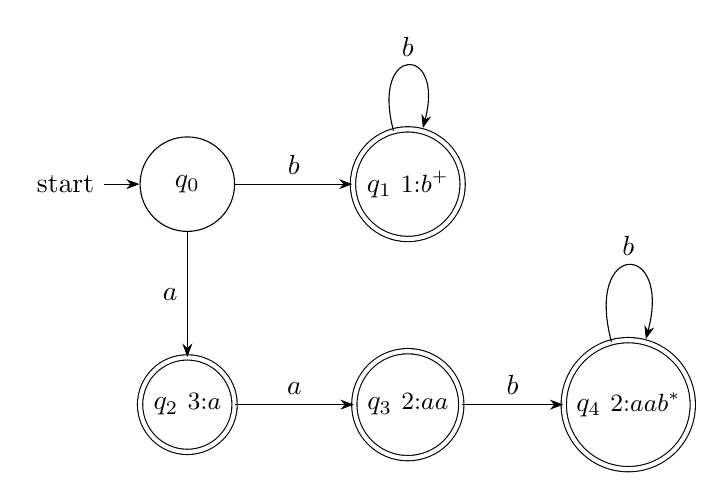
\begin{tikzpicture}[
    >=Stealth,
    node distance=28mm,
    every state/.style={minimum size=12mm},
    accepting/.style={double distance=1.5pt}
]

\node[state,initial] (q0) {$q_0$};
\node[state,accepting, right of=q0] (q1) {$q_1$ \small{1:$b^+$}};
\node[state,accepting, below of=q0] (q2) {$q_2$ \small{3:$a$}};
\node[state,accepting, right of=q2] (q3) {$q_3$ \small{2:$aa$}};
\node[state,accepting, right of=q3] (q4) {$q_4$ \small{2:$aab^*$}};

\path[->]
(q0) edge[above] node{$b$} (q1)
(q0) edge[left]  node{$a$} (q2)
(q1) edge[loop above] node{$b$} (q1)
(q2) edge[above] node{$a$} (q3)
(q3) edge[above] node{$b$} (q4)
(q4) edge[loop above] node{$b$} (q4);
\end{tikzpicture}
\end{center}

\subsubsection*{Trace Table}
\begin{center}
\begin{tabular}{|c|l|l|c|c|c|}
\hline
\textbf{\#} & \textbf{Remaining Input} & \textbf{Path (States)} & \textbf{Fallback} & \textbf{Lexeme} & \textbf{Out} \\ \hline
1 & aaabaabbababbb & $q_0 \xrightarrow{a} q_2 \xrightarrow{a} q_3 \xrightarrow{a} \text{Dead}$ & $q_3$ & aa & 2 \\ \hline
2 & abaabbababbb & $q_0 \xrightarrow{a} q_2 \xrightarrow{b} \text{Dead}$ & $q_2$ & a & 3 \\ \hline
3 & baabbababbb & $q_0 \xrightarrow{b} q_1 \xrightarrow{a} \text{Dead}$ & $q_1$ & b & 1 \\ \hline
4 & aabbababbb & $q_0 \xrightarrow{a} q_2 \xrightarrow{a} q_3 \xrightarrow{b} q_4 \xrightarrow{b} q_4 \xrightarrow{a} \text{Dead}$ & $q_4$ & aabb & 2 \\ \hline
5 & ababbb & $q_0 \xrightarrow{a} q_2 \xrightarrow{b} \text{Dead}$ & $q_2$ & a & 3 \\ \hline
6 & babbb & $q_0 \xrightarrow{b} q_1 \xrightarrow{a} \text{Dead}$ & $q_1$ & b & 1 \\ \hline
7 & abbb & $q_0 \xrightarrow{a} q_2 \xrightarrow{b} \text{Dead}$ & $q_2$ & a & 3 \\ \hline
8 & bbb & $q_0 \xrightarrow{b} q_1 \xrightarrow{b} q_1 \xrightarrow{b} q_1$ & End & bbb & 1 \\ \hline
\end{tabular}
\end{center}
\textbf{Final Printed Output:} 2 3 1 2 3 1 3 1


\subsection*{b. Second Regular Definition}
\textbf{Rules:} 
\begin{enumerate}
    \setcounter{enumi}{3}
    \item $(aa)^*b^* \rightarrow$ \texttt{printf("2")}
    \setcounter{enumi}{2}
    \item $a \rightarrow$ \texttt{printf("3")}
\end{enumerate}
\textbf{Priority:} $4 > 3$

\subsubsection*{State Diagram}
\begin{center}
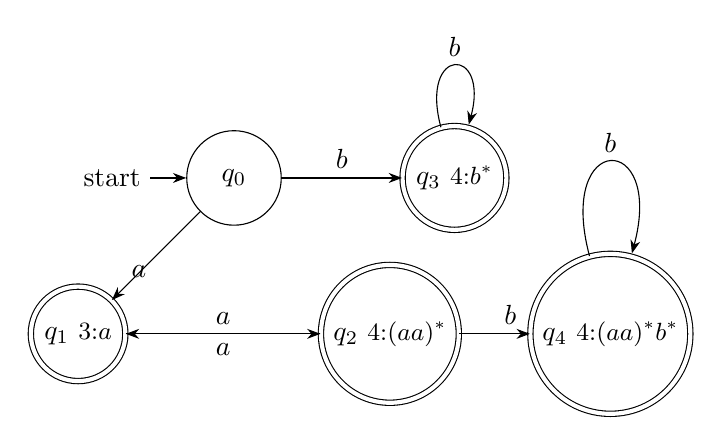
\begin{tikzpicture}[
    >=Stealth,
    node distance=28mm,
    every state/.style={minimum size=12mm},
    accepting/.style={double distance=1.5pt}
]

\node[state,initial] (q0) {$q_0$};
\node[state,accepting, below left of=q0] (q1) {$q_1$ \small{3:$a$}};
\node[state,accepting, below right of=q0] (q2) {$q_2$ \small{4:$(aa)^*$}};
\node[state,accepting, right of=q0] (q3) {$q_3$ \small{4:$b^*$}};
\node[state,accepting, right of=q2] (q4) {$q_4$ \small{4:$(aa)^*b^*$}};

\path[->]
(q0) edge[below left] node{$a$} (q1)
(q0) edge[above] node{$b$} (q3)
(q1) edge[below] node{$a$} (q2)
(q2) edge[above] node{$a$} (q1)
(q2) edge[above right] node{$b$} (q4)
(q3) edge[loop above] node{$b$} (q3)
(q4) edge[loop above] node{$b$} (q4);
\end{tikzpicture}
\end{center}

\subsubsection*{Trace Table}
\begin{center}
\begin{tabular}{|c|l|l|c|c|c|}
\hline
\textbf{\#} & \textbf{Remaining Input} & \textbf{Path (States)} & \textbf{Fallback} & \textbf{Lexeme} & \textbf{Out} \\ \hline
1 & aaabaabbababbb & $q_0 \xrightarrow{a} q_1 \xrightarrow{a} q_2 \xrightarrow{a} q_1 \xrightarrow{b} \text{Dead}$ & $q_2$ & aa & 2 \\ \hline
2 & abaabbababbb & $q_0 \xrightarrow{a} q_1 \xrightarrow{b} \text{Dead}$ & $q_1$ & a & 3 \\ \hline
3 & baabbababbb & $q_0 \xrightarrow{b} q_3 \xrightarrow{a} \text{Dead}$ & $q_3$ & b & 2 \\ \hline
4 & aabbababbb & $q_0 \xrightarrow{a} q_1 \xrightarrow{a} q_2 \xrightarrow{b} q_4 \xrightarrow{b} q_4 \xrightarrow{a} \text{Dead}$ & $q_4$ & aabb & 2 \\ \hline
5 & ababbb & $q_0 \xrightarrow{a} q_1 \xrightarrow{b} \text{Dead}$ & $q_1$ & a & 3 \\ \hline
6 & babbb & $q_0 \xrightarrow{b} q_3 \xrightarrow{a} \text{Dead}$ & $q_3$ & b & 2 \\ \hline
7 & abbb & $q_0 \xrightarrow{a} q_1 \xrightarrow{b} \text{Dead}$ & $q_1$ & a & 3 \\ \hline
8 & bbb & $q_0 \xrightarrow{b} q_3 \xrightarrow{b} q_3 \xrightarrow{b} q_3$ & End & bbb & 2 \\ \hline
\end{tabular}
\end{center}
\textbf{Final Printed Output:} 2 3 2 2 3 2 3 2

\newpage
% ---

\section*{3-4}
\textbf{Lexical Analyzers}

We would like to construct a tokenizer with the following specification.

Given an input stream of decimal digits, the stream should be split into segments and the outputs for consecutive segments should be produced in sequence. 

A segment is either a string of two digits, or a string of one digit if only one digit is available. 

If the segment is a string $d_1d_2$ of two digits, then the corresponding output depends on $d_2$: if $d_2 < 9$, the output is the two-digit decimal string representing $d_1d_2 +1$; if $d_2 = 9$, the output is $d_{10}$.

If the segment is a string of one digit $d$, then the output is $d$. Here are some illustrative examples.

\begin{table}[h]
\centering
\begin{tabular}{|c|c|c|}
\hline
\textbf{Input} & \multicolumn{2}{c|}{\textbf{Output}} \\ \hline
1235           & 13                & 36                \\ \hline
9807           & 99                & 08                \\ \hline
999            & 90                & 9                 \\ \hline
090            & 00                & 0                 \\ \hline
\end{tabular}
\end{table}

a. Give an action-augmented regular definition with rules describing input patterns and with
actions producing the corresponding outputs.

b. Draw the state diagram of the corresponding NFA.

c. Draw the state diagram of the corresponding fallback DFA with actions M.

d. Trace the operation of M on input 2003798, showing (i) the output and (ii) the sequence of states M goes through as it scans the input.


\begin{center}
  \underline{Solution:}
\end{center}

We define the patterns based on the digit sets $D = \{0, 1, \dots, 9\}$ and $D_{<9} = \{0, 1, \dots, 8\}$. The rules are prioritized by the \textbf{Longest Match} principle.

\begin{align*}
  1. \quad & D D_{<9} && \text{printf("\%02d", val(d1 d2) + 1)} \\
  2. \quad & D 9      && \text{printf("\%d0", d1)} \\
  3. \quad & D        && \text{printf("\%d", d)}
\end{align*}

\subsection*{b. State Diagram of the NFA}
The NFA transitions to different states to distinguish between the one-digit case and the two-digit cases.

\begin{center}
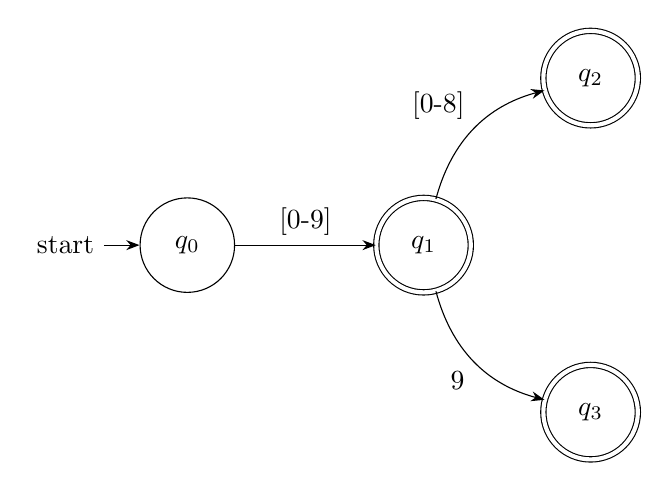
\begin{tikzpicture}[
    >=Stealth,
    node distance=30mm,
    every state/.style={minimum size=12mm},
    accepting/.style={double distance=1.5pt}
]

\node[state,initial] (q0) {$q_0$};
\node[state,accepting, right of=q0] (q1) {$q_1$};
\node[state,accepting, above right of=q1] (q2) {$q_2$};
\node[state,accepting, below right of=q1] (q3) {$q_3$};

\path[->]
(q0) edge[above] node{[0-9]} (q1)
(q1) edge[bend left, above left]  node{[0-8]} (q2)
(q1) edge[bend right, below left] node{9} (q3);

\end{tikzpicture}
\end{center}

\subsection*{c. Fallback DFA with Actions}
In the fallback DFA, every state reached by a digit is an accepting state. If the DFA reaches a dead end (e.g., trying to read a third digit), it falls back to the last seen accepting state.

\begin{center}
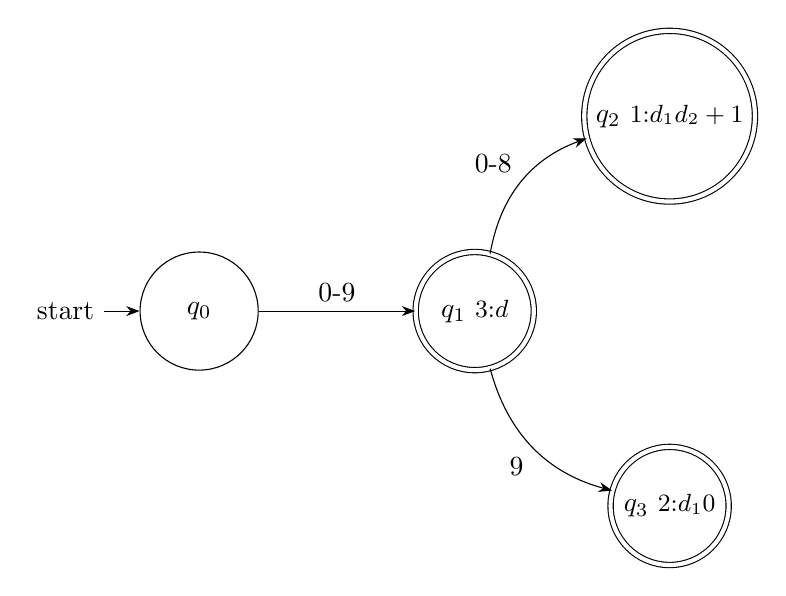
\begin{tikzpicture}[
    >=Stealth,
    node distance=35mm,
    every state/.style={minimum size=15mm},
    accepting/.style={double distance=1.5pt}
]

\node[state,initial] (q0) {$q_0$};
\node[state,accepting, right of=q0] (q1) {$q_1$ \small{3:$d$}};
\node[state,accepting, above right of=q1] (q2) {$q_2$ \small{1:$d_1d_2+1$}};
\node[state,accepting, below right of=q1] (q3) {$q_3$ \small{2:$d_10$}};

\path[->]
(q0) edge[above] node{0-9} (q1)
(q1) edge[bend left, above left] node{0-8} (q2)
(q1) edge[bend right, below left] node{9} (q3);

\end{tikzpicture}
\end{center}

\subsection*{d. Trace on input: 2003798}

\subsubsection*{(i) Output Trace Table}
\begin{center}
\begin{tabular}{|c|l|l|c|l|c|}
\hline
\textbf{Lexeme} & \textbf{Input} & \textbf{Path Taken} & \textbf{Rule} & \textbf{Calculation} & \textbf{Output} \\ \hline
1 & 20... & $q_0 \xrightarrow{2} q_1 \xrightarrow{0} q_2$ & 1 & $20 + 1$ & \textbf{21} \\ \hline
2 & 03... & $q_0 \xrightarrow{0} q_1 \xrightarrow{3} q_2$ & 1 & $03 + 1$ & \textbf{04} \\ \hline
3 & 79... & $q_0 \xrightarrow{7} q_1 \xrightarrow{9} q_3$ & 2 & $7 \rightarrow 70$ & \textbf{70} \\ \hline
4 & 8     & $q_0 \xrightarrow{8} q_1$ & 3 & 8 & \textbf{8} \\ \hline
\end{tabular}
\end{center}

\subsubsection*{(ii) Sequence of States}
The DFA moves through the following states (noting that the machine returns to $q_0$ after each lexeme is finalized):
$$ (q_0 \to q_1 \to q_2) \to (q_0 \to q_1 \to q_2) \to (q_0 \to q_1 \to q_3) \to (q_0 \to q_1) $$

\textbf{Final Printed Output:} 21 04 70 8
\newpage
% ---

\section*{3-5}
\textbf{Context-Free Grammars}

Give a context-free grammar (CFG) for each of the following languages:

a. $L = \{a^m b^n c^k | k = m + n; \: m, n, k \geq 0 \}$ over the alphabet $\Sigma = \{a, b, c\}$.

b. $L = \{a^m b^n | n \neq m\}$ over the alphabet $\Sigma = {a, b}$.

c. $L = \{w | w \text{ is a palindrome} \}$ over the alphabet $\Sigma = \{a, b, c\}$. 

(Note: A palindrome is a string that reads the same backwards as forwards.)

\begin{center}
  \underline{Solution:}
\end{center}

To solve these problems, we utilize the fundamental structure of context-free grammars (CFGs), which are defined by a set of variables, terminals, production rules, and a start variable. The following grammars leverage the recursive nature of CFGs to maintain counts and symmetry across different parts of a string.

\begin{enumerate}
    \item[\textbf{a.}] $L = \{a^m b^n c^k \mid k = m + n; \: m, n, k \geq 0 \}$ over $\Sigma = \{a, b, c\}$.
    
    To generate strings where the number of $c$'s equals the sum of $a$'s and $b$'s, we can think of the language as $a^m b^n c^{n+m}$. This can be structurally decomposed into matching the outer $a$'s with the trailing $c$'s, and then matching the inner $b$'s with the remaining $c$'s [1].
    
    \textbf{Grammar $G_a$}:
    \begin{align*}
        S &\to aSc \mid T \\
        T &\to bTc \mid \epsilon
    \end{align*}
    Here, $S$ recursively adds an $a$ to the front and a $c$ to the back, while $T$ does the same for $b$ and $c$ once all $a$'s are generated [1].

    \item[\textbf{b.}] $L = \{a^m b^n \mid n \neq m\}$ over $\Sigma = \{a, b\}$.
    
    This language consists of two cases: either there are more $a$'s than $b$'s ($m > n$) or more $b$'s than $a$'s ($n > m$). We can use the logic of generating equal numbers ($a^m b^m$) and then ensuring at least one extra symbol exists on the required side [1].
    
    \textbf{Grammar $G_b$}:
    \begin{align*}
        S &\to M \mid N \\
        E &\to aEb \mid \epsilon \\
        M &\to aM \mid aE \quad \text{(Case: } m > n\text{)} \\
        N &\to Nb \mid Eb \quad \text{(Case: } n > m\text{)}
    \end{align*}
    The variable $E$ generates equal numbers of $a$'s and $b$'s, while $M$ and $N$ force an imbalance by adding extra terminals to one side [1].

    \item[\textbf{c.}] $L = \{w \mid w \text{ is a palindrome} \}$ over $\Sigma = \{a, b, c\}$.
    
    A palindrome is constructed by ensuring that every symbol added to the front of the string is matched by the same symbol at the end. This symmetry is captured by recursive rules that wrap a smaller palindrome in matching terminal symbols [1].
    
    \textbf{Grammar $G_c$}:
    \begin{align*}
        S \to aSa \mid bSb \mid cSc \mid a \mid b \mid c \mid \epsilon
    \end{align*}
    The rules $aSa, bSb,$ and $cSc$ maintain the palindrome property, while $a, b, c,$ and $\epsilon$ serve as the base cases for odd-length and even-length palindromes, respectively [1].
\end{enumerate}

Building a CFG is like layering an onion; to ensure the outer layers match (like $a^m$ and $c^m$), you must define rules that grow the string from the center outward, maintaining the relationship between the symbols at the boundaries.
\newpage
% ---

\section*{3-6}
\textbf{Parse trees}

Consider the grammar:
\begin{align*}
  S &\rightarrow A1B \\
  A &\rightarrow 1A \:|\: 0 \\
  B &\rightarrow 0B \:|\: \epsilon
\end{align*}

Give a parse tree for each of the following strings:

a. 11101

b. 1010

c. 0100

\begin{center}
  \underline{Solution:}
\end{center}

The grammar provided is:
\begin{align*}
  S &\rightarrow A1B \\
  A &\rightarrow 1A \mid 0 \\
  B &\rightarrow 0B \mid \epsilon
\end{align*}

\subsection*{a. Parse tree for "11101"}
In this string, the terminal '1' from the $S$ rule is the final digit. The variable $A$ generates the prefix "1110", and $B$ generates the empty string $\epsilon$.

\begin{center}
\begin{forest}
  [$S$
    [$A$
      [1]
      [$A$
        [1]
        [$A$
          [1]
          [$A$ [0]]
        ]
      ]
    ]
    [1]
    [$B$ [$\epsilon$]]
  ]
\end{forest}
\end{center}

\subsection*{b. Parse tree for "1010"}
Here, the '1' from the $S$ rule is the second '1' in the string. $A$ generates "10", and $B$ generates "0".

\begin{center}
\begin{forest}
  [$S$
    [$A$
      [1]
      [$A$ [0]]
    ]
    [1]
    [$B$
      [0]
      [$B$ [$\epsilon$]]
    ]
  ]
\end{forest}
\end{center}

\subsection*{c. Parse tree for "0100"}
In this case, $A$ generates the leading "0", followed by the terminal '1' from the $S$ rule, and $B$ generates the trailing "00".

\begin{center}
\begin{forest}
  [$S$
    [$A$ [0]]
    [1]
    [$B$
      [0]
      [$B$
        [0]
        [$B$ [$\epsilon$]]
      ]
    ]
  ]
\end{forest}
\end{center}

\newpage
% ---

\section*{3-7}
\textbf{Derivations}

Consider the following context-free grammar:
\begin{align*}
  S \rightarrow SS+ \:|\: SS* \:|\: a
\end{align*}

and the string: $aa+a*$

a. Give a leftmost derivation for the string. Show the sequence of derivation rules applied.

b. Give a rightmost derivation for the string. Show the sequence of derivation rules applied.

c. Give a parse tree for the string.

\begin{center}
  \underline{Solution:}
\end{center}

The grammar rules are: 
(1) $S \to SS+$, (2) $S \to SS*$, (3) $S \to a$.

\subsection*{a. Leftmost Derivation}
A leftmost derivation always replaces the variable furthest to the left in the sentential form [1].

\begin{itemize}
    \item[] $S \Rightarrow SS*$ \hfill (Rule 2)
    \item[] $\phantom{S} \Rightarrow SS+ S*$ \hfill (Rule 1 applied to leftmost $S$)
    \item[] $\phantom{S} \Rightarrow aS+ S*$ \hfill (Rule 3 applied to leftmost $S$)
    \item[] $\phantom{S} \Rightarrow aa+ S*$ \hfill (Rule 3 applied to leftmost $S$)
    \item[] $\phantom{S} \Rightarrow aa+ a*$ \hfill (Rule 3 applied to leftmost $S$)
\end{itemize}

\textbf{Sequence of rules applied:} (2), (1), (3), (3), (3).

\subsection*{b. Rightmost Derivation}
A rightmost derivation always replaces the variable furthest to the right in the sentential form [1].

\begin{itemize}
    \item[] $S \Rightarrow SS*$ \hfill (Rule 2)
    \item[] $\phantom{S} \Rightarrow Sa*$ \hfill (Rule 3 applied to rightmost $S$)
    \item[] $\phantom{S} \Rightarrow SS+ a*$ \hfill (Rule 1 applied to rightmost $S$)
    \item[] $\phantom{S} \Rightarrow Sa+ a*$ \hfill (Rule 3 applied to rightmost $S$)
    \item[] $\phantom{S} \Rightarrow aa+ a*$ \hfill (Rule 3 applied to rightmost $S$)
\end{itemize}

\textbf{Sequence of rules applied:} (2), (3), (1), (3), (3).

\subsection*{c. Parse Tree}
The parse tree illustrates the derivation's hierarchy [1]. The root $S$ branches into the components of the multiplication rule, and the first $S$ sub-tree further branches into the addition components.



\begin{center}
\begin{forest}
  [$S$
    [$S$
        [$S$ [a]]
        [$S$ [a]]
        [+]
    ]
    [$S$ [a]]
    [*]
  ]
\end{forest}
\end{center}
\newpage
% ---

\section*{4-1}
\textbf{LL(1) Parsing}

Consider the following CFG:
\begin{align*}
  S \rightarrow SS+ \:|\: SS* \:|\: a
\end{align*}

a. Eliminate left recursion and left factor the grammar.

b. Compute first and follow sets for each non-terminal in the resulting grammar.

c. Build the predictive parsing table.

\begin{center}
  \underline{Solution:}
\end{center}
\newpage
% ---

\section*{4-2}
\textbf{LL(1) Parsing}

Consider the context-free grammar $G = (\{S, L,R\}, \{(, ),+, a\},R, S)$, where $R$ is the set of the following rules.
\begin{align*}
  S &\rightarrow (L) \:|\: a \\
  L &\rightarrow SR \\
  R &\rightarrow +SR \:|\: \epsilon
\end{align*}

a. Construct the LL(1) predictive parsing table for G.

b. Is G an LL(1) grammar? Why?
\begin{center}
  \underline{Solution:}
\end{center}
\newpage
% ---

\section*{4-3}
\textbf{LR(0) Automaton and SLR Parsing}

Consider the following grammar:
\begin{align*}
  S &\rightarrow Xa \\
  X &\rightarrow a \:|\: aXb
\end{align*}

a. Construct the LR(0) DFA of the grammar.

b. Construct the SLR parsing table.

c. Use the parsing table to simulate SLR parsing on the string: aaba

\begin{center}
  \underline{Solution:}
\end{center}

To solve this problem, we follow the standard procedures for augmenting a grammar, constructing an LR(0) automaton, and building an SLR parsing table.

\subsection*{(a) Construct the LR(0) DFA of the grammar}

We augment the grammar by adding a new start symbol $S'$ with the production
\[
S' \to S
\]
to provide a unique accept condition.

\subsubsection*{Augmented Grammar $G'$}
\[
\begin{array}{ll}
(0) & S' \to S \\
(1) & S \to Xa \\
(2) & X \to a \\
(3) & X \to aXb
\end{array}
\]

We now compute the LR(0) item sets using the \textbf{CLOSURE} and \textbf{GOTO} functions.

\[
I_0 = \text{CLOSURE}(\{S' \to \cdot S\})
     = \{S' \to \cdot S,\; S \to \cdot Xa,\; X \to \cdot a,\; X \to \cdot aXb\}
\]

\[
\begin{aligned}
I_1 &= \text{GOTO}(I_0,S) = \{S' \to S\cdot\} \\
I_2 &= \text{GOTO}(I_0,X) = \{S \to X\cdot a\} \\
I_3 &= \text{GOTO}(I_0,a) = \text{CLOSURE}(\{X \to a\cdot,\; X \to a\cdot Xb\}) \\
    &= \{X \to a\cdot,\; X \to a\cdot Xb,\; X \to \cdot a,\; X \to \cdot aXb\} \\
I_4 &= \text{GOTO}(I_2,a) = \{S \to Xa\cdot\} \\
I_5 &= \text{GOTO}(I_3,X) = \{X \to aX\cdot b\} \\
I_6 &= \text{GOTO}(I_5,b) = \{X \to aXb\cdot\}
\end{aligned}
\]

There is also a self-loop:
\[
\text{GOTO}(I_3,a)=I_3
\]

\subsection*{(b) SLR Parsing Table}

The FOLLOW sets are
\[
\text{FOLLOW}(S)=\{\$\}, \qquad
\text{FOLLOW}(X)=\{a,b\}.
\]

\[
\begin{array}{|c|ccc|cc|}
\hline
\textbf{State} & \multicolumn{3}{c|}{\textbf{ACTION}} & \multicolumn{2}{c|}{\textbf{GOTO}}\\
\cline{2-6}
 & a & b & \$ & S & X\\
\hline
0 & s3 &   &   & 1 & 2\\
1 &    &   & acc &   &  \\
2 & s4 &   &   &   &  \\
3 & s3/r2 & r2 &   &   & 5\\
4 &    &   & r1 &   &  \\
5 &    & s6 &   &   &  \\
6 & r3 & r3 &   &   &  \\
\hline
\end{array}
\]

\noindent
State 3 contains a shift/reduce conflict on input $a$.  
We choose **shift**.

\subsection*{(c) Parsing the string $aaba$}

\[
\begin{array}{|c|c|c|l|}
\hline
\textbf{Step} & \textbf{Stack} & \textbf{Input} & \textbf{Action}\\
\hline
1 & 0 & aaba\$ & s3\\
2 & 0\,3 & aba\$ & s3\\
3 & 0\,3\,3 & ba\$ & r2:\;X\to a\\
4 & 0\,3\,5 & ba\$ & s6\\
5 & 0\,3\,5\,6 & a\$ & r3:\;X\to aXb\\
6 & 0\,2 & a\$ & s4\\
7 & 0\,2\,4 & \$ & r1:\;S\to Xa\\
8 & 0\,1 & \$ & \textbf{accept}\\
\hline
\end{array}
\]

\subsection*{Conclusion}

The SLR parser correctly accepts the string \texttt{aaba}.  
During reductions (e.g., Step~5), the parser pops a number of states equal to the
length of the right-hand side and uses the GOTO table to push the next state
corresponding to the reduced nonterminal.


\newpage
% ---

\section*{4-4}
\textbf{LR(0) Automaton and SLR Parsing}

Consider the following grammar:
\begin{align*}
  S &\rightarrow aSc \:|\: Td \\
  T &\rightarrow Tb \:|\: b
\end{align*}

a. Construct the LR(0) DFA of the grammar.

b. Construct the SLR parsing table.

c. Is this grammar SLR ? Justify your answer.

d. Use the parsing table to simulate SLR parsing on the string: aabdcc

\begin{center}
  \underline{Solution:}
\end{center}

To solve this problem, we follow the standard procedure for augmenting a grammar, constructing an LR(0) automaton, and building an SLR parsing table.

\subsection*{(a) LR(0) Automaton}

We first augment the grammar by adding a new start symbol $S'$ and the production
\[
S' \to S .
\]

\paragraph{Augmented Grammar $G'$}
\[
\begin{array}{rcl}
(0) & S' &\to S \\
(1) & S  &\to aSc \\
(2) & S  &\to Td \\
(3) & T  &\to Tb \\
(4) & T  &\to b
\end{array}
\]

The LR(0) item sets are obtained using \textbf{CLOSURE} and \textbf{GOTO}.

\[
\begin{aligned}
I_0 &= \text{CLOSURE}(\{S' \to \cdot S\}) \\
    &= \{ S' \to \cdot S,\; S \to \cdot aSc,\; S \to \cdot Td,\; T \to \cdot Tb,\; T \to \cdot b \} \\[4pt]
I_1 &= \text{GOTO}(I_0,S) = \{ S' \to S \cdot \} \quad (\text{accept}) \\[4pt]
I_2 &= \text{GOTO}(I_0,a) \\
    &= \text{CLOSURE}(\{S \to a \cdot Sc\}) \\
    &= \{ S \to a \cdot Sc,\; S \to \cdot aSc,\; S \to \cdot Td,\; T \to \cdot Tb,\; T \to \cdot b \} \\[4pt]
I_3 &= \text{GOTO}(I_0,T) = \{ S \to T \cdot d,\; T \to T \cdot b \} \\[4pt]
I_4 &= \text{GOTO}(I_0,b) = \{ T \to b \cdot \} \\[4pt]
I_5 &= \text{GOTO}(I_2,S) = \{ S \to aS \cdot c \} \\[4pt]
I_6 &= \text{GOTO}(I_3,d) = \{ S \to Td \cdot \} \\[4pt]
I_7 &= \text{GOTO}(I_3,b) = \{ T \to Tb \cdot \} \\[4pt]
I_8 &= \text{GOTO}(I_5,c) = \{ S \to aSc \cdot \}
\end{aligned}
\]

Some important transitions:
\[
\text{GOTO}(I_2,a)=I_2,\qquad
\text{GOTO}(I_2,T)=I_3,\qquad
\text{GOTO}(I_2,b)=I_4 .
\]

\subsection*{(b) SLR Parsing Table}

The FOLLOW sets are:
\[
\text{FOLLOW}(S)=\{c,\$\}, \qquad \text{FOLLOW}(T)=\{d,b\}.
\]

\[
\begin{array}{|c|cccc|c|cc|}
\hline
\textbf{State} & \multicolumn{5}{c|}{\textbf{ACTION}} & \multicolumn{2}{c|}{\textbf{GOTO}}\\
\cline{2-8}
 & a & b & c & d & \$ & S & T\\
\hline
0 & s2 & s4 &   &   &   & 1 & 3\\
1 &    &    &   &   & acc &   &   \\
2 & s2 & s4 &   &   &     & 5 & 3\\
3 &    & s7 &   & s6 &     &   &   \\
4 &    & r4 &   & r4 &     &   &   \\
5 &    &    & s8 &   &     &   &   \\
6 &    &    & r2 &   & r2  &   &   \\
7 &    & r3 &   & r3 &     &   &   \\
8 &    &    & r1 &   & r1  &   &   \\
\hline
\end{array}
\]

\subsection*{(c) Is the Grammar SLR?}

Yes. The SLR table contains no shift/reduce or reduce/reduce conflicts. Each table entry has at most one action.

\subsection*{(d) Parsing \texttt{aabdcc}}

\[
\begin{array}{|c|l|l|l|}
\hline
\textbf{Step} & \textbf{Stack} & \textbf{Input} & \textbf{Action}\\
\hline
1 & 0 & aabdcc\$ & s2\\
2 & 0\,2 & abdcc\$ & s2\\
3 & 0\,2\,2 & bdcc\$ & s4\\
4 & 0\,2\,2\,4 & dcc\$ & r4: T\to b,\; \text{GOTO}(2,T)=3\\
5 & 0\,2\,2\,3 & dcc\$ & s6\\
6 & 0\,2\,2\,3\,6 & cc\$ & r2: S\to Td,\; \text{GOTO}(2,S)=5\\
7 & 0\,2\,2\,5 & cc\$ & s8\\
8 & 0\,2\,2\,5\,8 & c\$ & r1: S\to aSc,\; \text{GOTO}(2,S)=5\\
9 & 0\,2\,5 & c\$ & s8\\
10 & 0\,2\,5\,8 & \$ & r1: S\to aSc,\; \text{GOTO}(0,S)=1\\
11 & 0\,1 & \$ & \textbf{accept}\\
\hline
\end{array}
\]

\newpage
% ---

\section*{4-5}

Consider the following grammar:
\begin{align*}
  S &\rightarrow T,S \:|\: \epsilon \\
  T &\rightarrow int 0
\end{align*}

a. Construct the LR(0) DFA of the grammar.

b. Construct the SLR parsing table.

c. Is this grammar SLR ? Justify your answer.

d. Use the parsing table to simulate SLR parsing on the string: int 0 , int 0

\begin{center}
  \underline{Solution:}
\end{center}

\textbf{a. Construct the LR(0) DFA of the grammar.}

First, we augment the grammar with $S' \rightarrow S$ to create a unique starting point [1]. 
The augmented grammar $G'$ is:
(0) $S' \rightarrow S$, (1) $S \rightarrow T,S$, (2) $S \rightarrow \epsilon$, (3) $T \rightarrow int\;0$.

We compute the sets of items using the \textbf{CLOSURE} and \textbf{GOTO} functions [1, 2]:

\begin{itemize}
    \item \textbf{State $I_0$:} $\text{CLOSURE}(\{S' \rightarrow \cdot S\})$
    \begin{itemize}
        \item $S' \rightarrow \cdot S$
        \item $S \rightarrow \cdot T,S$
        \item $S \rightarrow \cdot$ \quad (reduction item for $S \rightarrow \epsilon$) [3]
        \item $T \rightarrow \cdot int\;0$ \quad (added because dot is before $T$) [1]
    \end{itemize}
    \item \textbf{State $I_1$:} $\text{GOTO}(I_0,S)=\{S' \rightarrow S\cdot\}$
    \item \textbf{State $I_2$:} $\text{GOTO}(I_0,T)=\{S \rightarrow T\cdot,S\}$
    \item \textbf{State $I_3$:} $\text{GOTO}(I_0,int)=\{T \rightarrow int\cdot 0\}$
    \item \textbf{State $I_4$:} $\text{GOTO}(I_2,{,})=\text{CLOSURE}(\{S \rightarrow T,\cdot S\})$
    \begin{itemize}
        \item $S \rightarrow T,\cdot S$
        \item $S \rightarrow \cdot T,S$
        \item $S \rightarrow \cdot$
        \item $T \rightarrow \cdot int\;0$
    \end{itemize}
    \item \textbf{State $I_5$:} $\text{GOTO}(I_3,0)=\{T \rightarrow int\;0\cdot\}$
    \item \textbf{State $I_6$:} $\text{GOTO}(I_4,S)=\{S \rightarrow T,S\cdot\}$
\end{itemize}

\textit{Note: Transitions for $T$ and $int$ from $I_4$ lead back to $I_2$ and $I_3$ respectively.}

\textbf{b. Construct the SLR parsing table.}

We need the \textbf{FOLLOW} sets to place reduction actions [4]:
\begin{itemize}
    \item $\text{FOLLOW}(S)=\{\$\}$
    \item $\text{FOLLOW}(T)=\{{,}\}$
\end{itemize}

\begin{center}
\begin{tabular}{|c|cccc|cc|}
\hline
\textbf{State} & \multicolumn{4}{c|}{\textbf{ACTION}} & \multicolumn{2}{c|}{\textbf{GOTO}} \\
\cline{2-7}
 & \textbf{int} & \textbf{0} & \textbf{,} & \textbf{\$} & \textbf{S} & \textbf{T} \\
\hline
0 & s3 & & & r2 & 1 & 2 \\
1 & & & & acc & & \\
2 & & & s4 & & & \\
3 & & s5 & & & & \\
4 & s3 & & & r2 & 6 & 2 \\
5 & & & r3 & & & \\
6 & & & & r1 & & \\
\hline
\end{tabular}
\end{center}

\textbf{c. Is this grammar SLR? Justify your answer.}

\textbf{Yes, this grammar is SLR.} A grammar is SLR if there are no conflicting actions in its parsing table [4]. In State 0 and State 4, we have both a shift action (on $int$) and a reduce action ($r2$ on $\$$). Because the terminal $int$ is not in $\text{FOLLOW}(S)$, these actions occupy different columns, and no shift/reduce or reduce/reduce conflicts occur [4, 5].

\textbf{d. Use the parsing table to simulate SLR parsing on the string: \texttt{int 0 , int 0}}

\begin{center}
\begin{tabular}{|l|l|l|l|}
\hline
\textbf{Step} & \textbf{Stack} & \textbf{Input} & \textbf{Action} \\
\hline
(1) & 0 & int 0 , int 0 \$ & shift to 3 \\
(2) & 0\;3 & 0 , int 0 \$ & shift to 5 \\
(3) & 0\;3\;5 & , int 0 \$ & reduce by $T \rightarrow int\;0$ ($r3$) \\
(4) & 0\;2 & , int 0 \$ & shift to 4 \\
(5) & 0\;2\;4 & int 0 \$ & shift to 3 \\
(6) & 0\;2\;4\;3 & 0 \$ & shift to 5 \\
(7) & 0\;2\;4\;3\;5 & \$ & \textbf{ERROR} \\
\hline
\end{tabular}
\end{center}

\textbf{Justification of Error:} The simulation results in an error at step 7 because $ACTION[5,\$]$ is empty. In this grammar, every $T$ ($int\;0$) must be followed by a comma to satisfy $S \rightarrow T,S$, or the string must be empty ($\epsilon$) to satisfy $S \rightarrow \epsilon$ [3, 6]. The provided string \texttt{int 0 , int 0} is missing a trailing comma and is therefore not in the language defined by the grammar.
\newpage
% ---

\section*{4-6}
\textbf{LR(0) Automaton and SLR Parsing}

Consider the following grammar:
\begin{align*}
  S &\rightarrow AaAb \:|\: BbBa \\
  A &\rightarrow \epsilon \\
  B &\rightarrow \epsilon
\end{align*}

Is it LL(1)? Is it SLR?

\begin{center}
  \underline{Solution:}
\end{center}

\textbf{Is it LL(1)?}

\textbf{Yes, the grammar is LL(1).} 

Why it's LL(1): A top-down parser can easily distinguish between starting with A or B based on whether the first token it sees is a or b.
\newline

\textbf{Is it SLR?}

\textbf{No, the grammar is not SLR.} 

Why it fails SLR(1): The SLR parser will reach a state where it needs to decide whether to reduce $A \rightarrow \epsilon$ or $B \rightarrow \epsilon$. Because both a and b can follow these non-terminals in different parts of the grammar, the FOLLOW sets overlap, creating a conflict the SLR parser cannot resolve.
\newpage
% ---

\section*{4-7}
Consider the following grammar:
\begin{align*}
  S &\rightarrow SA \:|\: A \\
  A &\rightarrow a
\end{align*}

Show that the grammar is SLR but not LL(1).

\begin{center}
  \underline{Solution:}
\end{center}

\textbf{The Grammar is Not LL(1)}

The grammar cannot be LL(1) if it is left-recursive.

In the production $S \rightarrow SA$, the non-terminal $S$ appears as the very first symbol on the right-hand side. This creates an infinite loop for a top-down parser: to parse $S$, it first tries to parse $S$, which requires it to parse $S$ again, and so on.

Formal LL(1) Conflict: For a grammar to be LL(1), the FIRST sets of the productions for a non-terminal must be disjoint.

$FIRST(SA)=FIRST(S)=\{a\}$

$FIRST(A)=\{a\}$

Since the FIRST sets for both productions of $S$ overlap $a \in \{ a \} \cap \{ a \}$, the parser cannot decide which production to choose based on one token of lookahead.
\newline

\textbf{The Grammar is SLR}

To prove a grammar is SLR, we must construct the SLR parsing table and verify that there are no conflicts.
\newpage
% ---

\section*{4-8}
Consider the following grammar:
\begin{align*}
  A &\rightarrow BCD \\
  B &\rightarrow Bb \:|\: \epsilon \\
  C &\rightarrow cC \:|\: \epsilon \\
  D &\rightarrow d
\end{align*}

Is this grammar LR(0)?

\begin{center}
  \underline{Solution:}
\end{center}

\textbf{The Augmented Grammar}

First, we add a new starting production to create a clear "Accept" state: 
\begin{align*}
0. A^\prime &\rightarrow A \\  
1. A &\rightarrow BCD \\
2. B &\rightarrow Bb \\
3. B &\rightarrow \epsilon \\
4. C &\rightarrow cC \\
5. C &\rightarrow \epsilon \\
6. D &\rightarrow d
\end{align*}


\textbf{Constructing State $I_0$}

$I_0 = \{ A^\prime \rightarrow \cdot A, A \rightarrow \cdot BCD, B \rightarrow \cdot Bb, B \rightarrow \cdot \}$
\newline

\textbf{Identifying the LR(0) Conflict}

An LR(0) grammar cannot have any state that contains a completed reduction alongside another item.

In State $I_0$, we have a clear Shift/Reduce conflict:

Reduce Item: $B \rightarrow \cdot$

Shift Items: $A \rightarrow \cdot BCD$ (requires a shift on B) and $B \rightarrow \cdot Bb$ (requires a shift on B).

In an LR(0) parser, if a state contains $B \rightarrow \cdot$, the parser is told to "Reduce by $B \rightarrow \epsilon$" regardless of the next input token. However, in the same state, the parser is also told to "Shift" if it sees symbols that could start B. This ambiguity makes the grammar not LR(0).
\newpage
% ---

\section*{4-9}
\textbf{SLR and LALR Parsing}

Show that the following grammar is LALR but not SLR.
\begin{align*}
  S &\rightarrow Aa \:|\: bAc \:|\: dc \:|\: bda \\
  A &\rightarrow d
\end{align*}

Trace the operation of an LALR parser on input sentence

\begin{center}
  \underline{Solution:}
\end{center}

To solve this problem, we will apply the concepts of core-equivalence and lookahead propagation that we've discussed. This specific grammar is a classic example used to show how SLR's reliance on global FOLLOW sets can lead to conflicts that more advanced parsers, like LALR, can resolve by tracking context.

\subsection*{1. Why the grammar is NOT SLR}

To determine if the grammar is SLR, we first compute the FOLLOW sets for the non-terminals:
\begin{itemize}
\item $\text{FOLLOW}(S)=\{\$\}$
\item $\text{FOLLOW}(A)=\{a,c\}$ \quad (from $S \to Aa$ and $S \to bAc$)
\end{itemize}

Now, let's look at the LR(0) item sets where conflicts arise:

\medskip
\textbf{State $I_2$ (reached from $I_0$ on terminal $d$):}
\begin{align*}
S &\to d.c \\
A &\to d.
\end{align*}

In SLR, for the item $A \to d.$, we call for a reduction if the next input symbol is in $\text{FOLLOW}(A)$, which is $\{a,c\}$.  
However, the item $S \to d.c$ calls for a shift on terminal $c$.  
Because $c \in \text{FOLLOW}(A)$, there is a \textbf{shift--reduce conflict} on input $c$.

\medskip
\textbf{State $I_3$ (reached from $I_1$ on terminal $d$, where $I_1=\text{GOTO}(I_0,b)$):}
\begin{align*}
S &\to bd.a \\
A &\to d.
\end{align*}

Similarly, $\text{FOLLOW}(A)$ includes $a$.  
The item $S \to bd.a$ calls for a shift on $a$, while $A \to d.$ calls for a reduction on $a$.  
This is a second \textbf{shift--reduce conflict}.  
Because of these conflicts, the grammar is not SLR.

\subsection*{2. Why the grammar IS LALR}

LALR resolves these conflicts by using specific lookaheads rather than the broad FOLLOW set.  
Let us examine the LR(1) items for these states.

\medskip
\textbf{In State $I_2$ (prefix $d$):}  
The item $A \to .d$ is generated by $S \to .Aa$.  
The lookahead for this $A$ production is
\[
\text{FIRST}(a\$)=\{a\}.
\]

\begin{align*}
S &\to d.c,\ \ \$ \\
A &\to d.,\ \ a
\end{align*}

The parser only reduces $A \to d$ if the next symbol is $a$.  
If the next symbol is $c$, it correctly chooses to shift for $S \to dc$.  
\textbf{No conflict.}

\medskip
\textbf{In State $I_3$ (prefix $bd$):}  
The item $A \to .d$ is generated by $S \to b.Ac$.  
The lookahead for this $A$ production is
\[
\text{FIRST}(c\$)=\{c\}.
\]

\begin{align*}
S &\to bd.a,\ \ \$ \\
A &\to d.,\ \ c
\end{align*}

The parser only reduces $A \to d$ if the next symbol is $c$.  
If the next symbol is $a$, it correctly chooses to shift for $S \to bda$.  
\textbf{No conflict.}

Since the LR(1) automaton has no conflicts, the LALR automaton (which merges states with the same core) also has no conflicts in this case.  
Therefore, the grammar is \textbf{LALR}.

\subsection*{3. Tracing the LALR Parser on ``bdc''}

We trace the operation on the string \textbf{``bdc''} to show how the parser distinguishes between the different roles of the terminal $d$.

\begin{center}
\begin{tabular}{|l|l|l|l|}
\hline
\textbf{Stack} & \textbf{Input} & \textbf{Action} & \textbf{Explanation} \\
\hline
0 & bdc\$ & shift $I_1$ & Shift $b$. \\
\hline
0 b 1 & dc\$ & shift $I_3$ & Shift $d$. \\
\hline
0 b 1 d 3 & c\$ & reduce $A \to d$ & \textbf{Lookahead is $c$}, so reduce $A \to d$ (Rule 5). \\
\hline
0 b 1 A 4 & c\$ & shift 5 & GOTO(1,$A$) leads to state 4. Shift $c$. \\
\hline
0 b 1 A 4 c 5 & \$ & reduce $S \to bAc$ & Reduce by Rule 2. \\
\hline
0 S 6 & \$ & acc & Accept string. \\
\hline
\end{tabular}
\end{center}
\newpage
% ---

\section*{4-10}
\textbf{LALR and LR(1) Parsing}

Show that the following grammar is LR(1) but not LALR.
\begin{align*}
  S &\rightarrow Aa \:|\: bAc \:|\: Bc \:|\: bBa \\
  A &\rightarrow d \\
  B &\rightarrow d
\end{align*}

\begin{center}
  \underline{Solution:}
\end{center}

To solve this problem, we must look at how Canonical LR(1) and LALR handle context differently.

As we discussed, LALR is more efficient because it merges states with the same ``core,'' but this merger can sometimes introduce reduce/reduce conflicts that were not present in the original LR(1) automaton.

Consider the augmented grammar $G'$:
\[
\begin{aligned}
(0)\;& S' \to S \\
(1)\;& S \to Aa \\
(2)\;& S \to bAc \\
(3)\;& S \to Bc \\
(4)\;& S \to bBa \\
(5)\;& A \to d \\
(6)\;& B \to d
\end{aligned}
\]

\subsection*{1. Showing the Grammar is LR(1)}

In a Canonical LR(1) parser, states are distinguished by their lookaheads. Let us examine the two critical paths for the terminal $d$.

\paragraph{Path 1: After reading prefix $d$}

The parser is at the start of either $S \to Aa$ or $S \to Bc$.
\begin{itemize}
\item For $S \to .Aa,\ \$ $, the closure gives $A \to .d,\ a$.
\item For $S \to .Bc,\ \$ $, the closure gives $B \to .d,\ c$.
\end{itemize}

This results in an LR(1) state (call it $I_x$):
\[
I_x = \{[A \to d., a],\; [B \to d., c]\}.
\]
In this state, if the lookahead is $a$, the parser reduces $d$ to $A$; if it is $c$, it reduces $d$ to $B$. There is no conflict.

\paragraph{Path 2: After reading prefix $bd$}

The parser is at the start of $S \to b.Ac$ or $S \to b.Ba$.
\begin{itemize}
\item For $S \to b.Ac,\ \$ $, the closure gives $A \to .d,\ c$.
\item For $S \to b.Ba,\ \$ $, the closure gives $B \to .d,\ a$.
\end{itemize}

This produces a different LR(1) state (call it $I_y$):
\[
I_y = \{[A \to d., c],\; [B \to d., a]\}.
\]
Again, the lookaheads clearly distinguish which reduction to take, so no conflict exists in LR(1).

\subsection*{2. Showing the Grammar is \emph{Not} LALR}

The LALR construction merges states that are core-equivalent, meaning they have the same LR(0) items regardless of lookaheads.

States $I_x$ and $I_y$ share the same core:
\[
\{A \to d.,\; B \to d.\}.
\]
When merged into a single LALR state $I_{xy}$, the lookaheads are unioned:
\[
I_{xy} = \{[A \to d., \{a,c\}],\; [B \to d., \{a,c\}]\}.
\]

Now, if the parser is in state $I_{xy}$ and the next input symbol is $a$, it has two possible reductions:
\begin{enumerate}
\item Reduce by $A \to d$ (since $a \in \text{Lookahead}(A \to d)$),
\item Reduce by $B \to d$ (since $a \in \text{Lookahead}(B \to d)$).
\end{enumerate}

This is a reduce/reduce conflict. Therefore, although the grammar is LR(1), it is not LALR.

\newpage
% ---

\section*{4-11}
\textbf{Canonical LR(1) Parsing}

Consider the following grammar:
\begin{align*}
  S &\rightarrow Xa \\
  X &\rightarrow a \:|\: aXb
\end{align*}

a. Compute the LR(1) item set and construct the LR(1) DFA of the grammar.

b. Construct the canonical LR(1) parsing table.

c. Use the parsing table to simulate canonical LR(1) parsing on the string: aaba

\begin{center}
  \underline{Solution:}
\end{center}

To solve this problem, we follow the formal procedures for augmenting the grammar, constructing the canonical collection of LR(1) item sets, building the parsing table, and tracing the input string [1, 2].

The grammar is:
\begin{enumerate}
    \item $S \to Xa$
    \item $X \to a$
    \item $X \to aXb$
\end{enumerate}

First, we augment the grammar with a new start symbol $S'$ and an endmarker $\$$ [3, 4]: \\
(0) $S' \to S, \$$

\subsection*{a. LR(1) Item Sets and DFA}

We compute the sets of items using the $\text{CLOSURE}$ and $\text{GOTO}$ functions [3, 5]. 

\noindent \textbf{$I_0$ (Initial State):} \\
$\text{CLOSURE}(\{[S' \to .S, \$]\})$:
\begin{enumerate}
    \item $[S' \to .S, \$]$
    \item $[S \to .Xa, \$]$ (Since $\text{FIRST}(\epsilon a \$) = \{a\}$ -- \textit{Correction: lookahead is 'a'})
    \item $[X \to .a, a]$ (Since $\text{FIRST}(a \$) = \{a\}$)
    \item $[X \to .aXb, a]$ (Since $\text{FIRST}(a \$) = \{a\}$)
\end{enumerate}
\textbf{$I_0 = \{[S' \to .S, \$], [S \to .Xa, \$], [X \to .a, a], [X \to .aXb, a]\}$}

\vspace{1em}
\noindent \textbf{$I_1 = \text{GOTO}(I_0, S) = \{[S' \to S., \$]\}$}

\noindent \textbf{$I_2 = \text{GOTO}(I_0, X) = \{[S \to X.a, \$]\}$}

\noindent \textbf{$I_3 = \text{GOTO}(I_0, a)$:} \\
Core: $[X \to a., a]$ and $[X \to a.Xb, a]$ \\
$\text{CLOSURE}$ of $[X \to a.Xb, a]$ adds $X$ productions with lookahead $\text{FIRST}(ba) = \{b\}$: \\
\textbf{$I_3 = \{[X \to a., a], [X \to a.Xb, a], [X \to .a, b], [X \to .aXb, b]\}$}

\noindent \textbf{$I_4 = \text{GOTO}(I_2, a) = \{[S \to Xa., \$]\}$}

\noindent \textbf{$I_5 = \text{GOTO}(I_3, X) = \{[X \to aX.b, a]\}$}

\noindent \textbf{$I_6 = \text{GOTO}(I_3, a)$:} \\
Core: $[X \to a., b]$ and $[X \to a.Xb, b]$ \\
$\text{CLOSURE}$ adds $X$ productions with lookahead $\text{FIRST}(bb) = \{b\}$: \\
\textbf{$I_6 = \{[X \to a., b], [X \to a.Xb, b], [X \to .a, b], [X \to .aXb, b]\}$}

\noindent \textbf{$I_7 = \text{GOTO}(I_5, b) = \{[X \to aXb., a]\}$}

\noindent \textbf{$I_8 = \text{GOTO}(I_6, X) = \{[X \to aX.b, b]\}$}

\noindent \textbf{$I_9 = \text{GOTO}(I_8, b) = \{[X \to aXb., b]\}$}

\textit{Transitions: $\text{GOTO}(I_6, a) = I_6$.}

\subsection*{b. Canonical LR(1) Parsing Table}



We fill the table based on the items in each state [2, 6]. For the conflict in State 3, we follow the standard convention of shifting over reducing.

\begin{center}
\begin{tabular}{|c|c|c|c|c|c|}
\hline
\textbf{State} & \multicolumn{3}{c|}{\textbf{ACTION}} & \multicolumn{2}{c|}{\textbf{GOTO}} \\ \cline{2-6}
 & \textbf{a} & \textbf{b} & \textbf{\$} & \textbf{S} & \textbf{X} \\ \hline
0 & s3 & & & 1 & 2 \\ \hline
1 & & & acc & & \\ \hline
2 & s4 & & & & \\ \hline
3 & s6 / r2* & & & & 5 \\ \hline
4 & & & r1 & & \\ \hline
5 & & s7 & & & \\ \hline
6 & s6 & r2 & & & 8 \\ \hline
7 & r3 & & & & \\ \hline
8 & & s9 & & & \\ \hline
9 & & r3 & & & \\ \hline
\end{tabular}
\end{center}
\textit{*Note: Conflict in State 3. We use s6 for the simulation [7].}

\subsection*{c. Simulation on string "aaba"}

\begin{center}
\begin{tabular}{|l|l|c|l|}
\hline
\textbf{Stack} & \textbf{Input} & \textbf{Action} & \textbf{Explanation} \\ \hline
0 & aaba\$ & s3 & Shift 'a', go to state 3. \\ \hline
0 a 3 & aba\$ & s6 & Shift 'a' (resolving conflict), go to state 6. \\ \hline
0 a 3 a 6 & ba\$ & r2 & Reduce by $X \to a$. Pop 6. $\text{GOTO}(3, X)=5$. \\ \hline
0 a 3 X 5 & ba\$ & s7 & Shift 'b', go to state 7. \\ \hline
0 a 3 X 5 b 7 & a\$ & r3 & Reduce by $X \to aXb$. Pop 7, 5, 3. $\text{GOTO}(0, X)=2$. \\ \hline
0 X 2 & a\$ & s4 & Shift 'a', go to state 4. \\ \hline
0 X 2 a 4 & \$ & r1 & Reduce by $S \to Xa$. Pop 4, 2. $\text{GOTO}(0, S)=1$. \\ \hline
0 S 1 & \$ & acc & Accept string. \\ \hline
\end{tabular}
\end{center}
\newpage
% ---

\section*{4-12}
\textbf{LALR Parsing}

Consider the context-free grammar $G = (\{S, T\}, \{0, 1\},R, S)$, where $R$ is the set of the following rules.
\begin{align*}
  S &\rightarrow 0T \\
  T &\rightarrow 1ST \\
  T &\rightarrow 0
\end{align*}

The LALR automaton of G consists of the following states.

\begin{align*}
I_0 : S^{\prime} \rightarrow .S, \$ \\
S \rightarrow .0T, \$ \\\\
I_1 : S^{\prime} \rightarrow S., \$ \\\\
I_2 : S \rightarrow 0.T, \$/1/0 \\
T \rightarrow .1ST, \$/1/0 \\
T \rightarrow .0, \$/1/0 \\\\
I_3 : S \rightarrow 0T., \$/1/0 \\\\
I_4 : T \rightarrow 1.ST, \$/1/0 \\
S \rightarrow .0T, 1/0 \\\\
I_5 : T \rightarrow 0., \$/1/0 \\\\
I_6 : T \rightarrow 1S.T, \$/1/0 \\
T \rightarrow .1ST, \$/1/0 \\
T \rightarrow .0, \$/1/0 \\\\
I_7 : T \rightarrow 1ST., \$/1/0
\end{align*}

a. With $\delta$ being the transition function of the LALR automaton, which states are $\delta(I_2, 0)$ and $\delta(I_6, 1)$?

b. Construct the LALR parsing table for G.

c. Trace the operation of the LR parsing algorithm on input 01000 using the LALR parsing table from part (2) above. (Show the sequence of stack, input, and chosen action.)


\begin{center}
  \underline{Solution:}
\end{center}

Using the provided grammar and LALR automaton states, we will determine the transitions, construct the parsing table, and trace the input string.

The grammar rules are:
\[
(1)\; S \to 0T \qquad
(2)\; T \to 1ST \qquad
(3)\; T \to 0
\]

\subsection*{a. Transition Functions}

The transition function $\delta$ (or GOTO) for an LALR automaton is determined by moving the dot over the specified symbol in the items of a state and finding the resulting set of items.

\begin{itemize}
\item \textbf{$\delta(I_2,0)$:}
In state $I_2$, we have the item $[T \to .0,\$/1/0]$.
Moving the dot over $0$ results in the item $[T \to 0.,\$/1/0]$.
This set matches state $\mathbf{I_5}$.

\item \textbf{$\delta(I_6,1)$:}
In state $I_6$, we have the item $[T \to .1ST,\$/1/0]$.
Moving the dot over $1$ results in the item $[T \to 1.ST,\$/1/0]$.
This core matches state $\mathbf{I_4}$.
\end{itemize}

\subsection*{b. LALR Parsing Table}

The ACTION table is filled by identifying shifts based on terminal transitions and reductions based on completed items $(A\to\alpha.)$ and their lookaheads.
The GOTO table is filled using transitions on non-terminals.

\begin{center}
\begin{tabular}{|c|c|c|c|c|c|}
\hline
\textbf{State} & \multicolumn{3}{c|}{\textbf{ACTION}} & \multicolumn{2}{c|}{\textbf{GOTO}}\\
\cline{2-6}
 & \textbf{0} & \textbf{1} & \textbf{\$} & \textbf{S} & \textbf{T}\\
\hline
0 & s2 &   &    & 1 &   \\
\hline
1 &    &   & acc &   &   \\
\hline
2 & s5 & s4 &    &   & 3 \\
\hline
3 & r1 & r1 & r1 &   &   \\
\hline
4 & s2 &   &    & 6 &   \\
\hline
5 & r3 & r3 & r3 &   &   \\
\hline
6 & s5 & s4 &    &   & 7 \\
\hline
7 & r2 & r2 & r2 &   &   \\
\hline
\end{tabular}
\end{center}

\textit{Table Logic:}
\begin{itemize}
\item \textbf{State 0:} Transitions on `0' lead to $I_2$ (s2). Transition on `S' leads to $I_1$.
\item \textbf{State 2:} Transitions on `0' lead to $I_5$ (s5) and on `1' to $I_4$ (s4). Transition on `T' leads to $I_3$.
\item \textbf{State 3:} Contains $[S \to 0T.,\$/1/0]$, calling for reduction by rule 1 on all lookaheads.
\item \textbf{State 4:} Transition on `0' leads to $I_2$ (s2). Transition on `S' leads to $I_6$.
\item \textbf{State 5:} Contains $[T \to 0.,\$/1/0]$, calling for reduction by rule 3.
\item \textbf{State 6:} Transitions on `0' lead to $I_5$ (s5) and on `1' to $I_4$ (s4). Transition on `T' leads to $I_7$.
\item \textbf{State 7:} Contains $[T \to 1ST.,\$/1/0]$, calling for reduction by rule 2.
\end{itemize}

\subsection*{c. Trace on input ``01000''}

The simulation follows the standard LR parsing algorithm.

\begin{center}
\begin{tabular}{|l|r|c|l|}
\hline
\textbf{Stack} & \textbf{Input} & \textbf{Action} & \textbf{Explanation}\\
\hline
0 & 01000\$ & s2 & Shift 0, go to state 2.\\
\hline
0\;0\;2 & 1000\$ & s4 & Shift 1, go to state 4.\\
\hline
0\;0\;2\;1\;4 & 000\$ & s2 & Shift 0, go to state 2.\\
\hline
0\;0\;2\;1\;4\;0\;2 & 00\$ & s5 & Shift 0, go to state 5.\\
\hline
0\;0\;2\;1\;4\;0\;2\;0\;5 & 0\$ & r3 & $T\to0$. Pop $(0,5)$. GOTO$(2,T)=3$.\\
\hline
0\;0\;2\;1\;4\;0\;2\;T\;3 & 0\$ & r1 & $S\to0T$. Pop $(0,2,T,3)$. GOTO$(4,S)=6$.\\
\hline
0\;0\;2\;1\;4\;S\;6 & 0\$ & s5 & Shift 0, go to state 5.\\
\hline
0\;0\;2\;1\;4\;S\;6\;0\;5 & \$ & r3 & $T\to0$. Pop $(0,5)$. GOTO$(6,T)=7$.\\
\hline
0\;0\;2\;1\;4\;S\;6\;T\;7 & \$ & r2 & $T\to1ST$. Pop $(1,4,S,6,T,7)$. GOTO$(2,T)=3$.\\
\hline
0\;0\;2\;T\;3 & \$ & r1 & $S\to0T$. Pop $(0,2,T,3)$. GOTO$(0,S)=1$.\\
\hline
0\;S\;1 & \$ & acc & String accepted.\\
\hline
\end{tabular}
\end{center}

\newpage

\end{document}